\section{Messwerterfassung mit Arduino}
\label{sec:MesswerterfassungArduino}
In diesem Unterkapitel werden die verschiedenen Messgrößen und die allgemeine Messwerterfassung dargestellt, sowie das Programm das zur Planung und Gestaltung der Platinen genutzt wurde.
\paragraph{Messgrößen} Der Sensorknoten soll nach seiner Fertigstellung verschiedene Messgrößen ermitteln können. Aus diesem Grund muss zunächst festgelegt werden, welche Messgrößen bestimmt werden sollen. Für diese Messgrößen müssen dann für die Umsetzung passende Sensoren gefunden werden. Folgende Messgrößen sollte der Sensorknoten bestimmen können:
\begin{itemize}
	\item Temperatur
	\begin{itemize}
		\item Lufttemperatur
		\item Bodentemperatur 
	\end{itemize}
	\item Luftfeuchtigkeit
	\item Luftdruck
	\item Beleuchtungsstärke
	\item Bodenfeuchtigkeit
	\item Erkennung von Bewegung um den Sensorknoten
	\item Erkennung ob ein Fenster/Tür geschlossen oder geöffnet ist
\end{itemize}
\paragraph{Ablauf der Messwerterfassung} Die Messwerterfassung soll in zyklischen Abständen erfolgen. Um das Mesh-Netz nicht mit Nachrichten zu überlasten werden nur jede Minute alle Messwerte gemessen und in das Netzwerk gesendet. Jeder Messwert hat eine eindeutige ID. Mit Hilfe dieser ID wird angeben welche Einheit der Messwert hat. 

Die verschiedenen Messwerte werden mit mehreren Sensoren ermittelt. In jedem Zyklus werden die Sensorwerte in der gleichen Reihenfolge bestimmt. Zusätzlich zur Ermittlung der Messwert muss überprüft werden ob der Messwert überhaupt bestimmt werden kann. Beispiele dafür,  dass der Messwert nicht bestimmt werden kann ist, dass der Sensor nicht angeschlossen ist oder der Sensor nicht mehr Ordnungsgemäß funktioniert. 

Nachdem der Sensorwert ermittelt wurde werden die Werte in ein Paket zusammengefasst und versendet.  
\paragraph{Eagle Autodesk} Für die Entwicklung des Schaltplans und der Platine, auf der die Sensoren,  das Funkmodul und der Arduino aufgebracht werden sollen, wird Eagle von der Firma Autodesk eingesetzt. Bei Eagle handelt es sich um ein \ac{PCB}-Designer zum Erstellen von Layouts für Platinen (siehe Screenshot \ref{img:EagleAutodesk}). In der Studienarbeit wurde die Version 8.0.2 verwendet. Eagle ist für Windows, Mac und Linux Systeme erhältlich. Eagle besitzt verschiedene Lizenzversionen, die teilweise kostenlos zur Verfügung stehen. Die kostenlose Version ist für die nicht kommerzielle Nutzung lizenziert. Diese enthält einige Einschränkungen. So können maximal zwei Schaltpläne für ein Projekt verwendet werden, es werden maximal zwei Schichten unterstützt und die Größe der Platine ist auf 80 $cm^{2}$ beschränkt.

Eagle selbst besteht aus mehreren Komponenten, dazu gehören ein Schaltplan-Editor, ein Layout Editor und \ac{PCB}-Libraries. Der Schaltplan Editor ermöglicht es einen Schaltplan zu zeichnen. Hierfür können entweder Standardelemente verwendetet werden oder über Libraries neue elektronische Bauteile genutzt werden. Zusätzlich bietet Eagle einen ‚Electrical Rule Checking‘ an, mit dessen Hilfe können Fehler im Schaltplan gefunden werde. Durch eine direkte Verknüpfung zwischen Schaltplan und Layout können effizient Platinen entwickelt werden. Mit Hilfe des Layouters lassen sich Bauteile einfach platzieren und mit dem Autorouter lassen sich die die einzelnen Bauteile mit Leiterbahnen verbinden. Das Design kann anschließend nach definierten Regeln, wie zum Beispiel Abstand zwischen den Leiterbahnen, überprüft werden. 
\begin{figure}
	\centering
	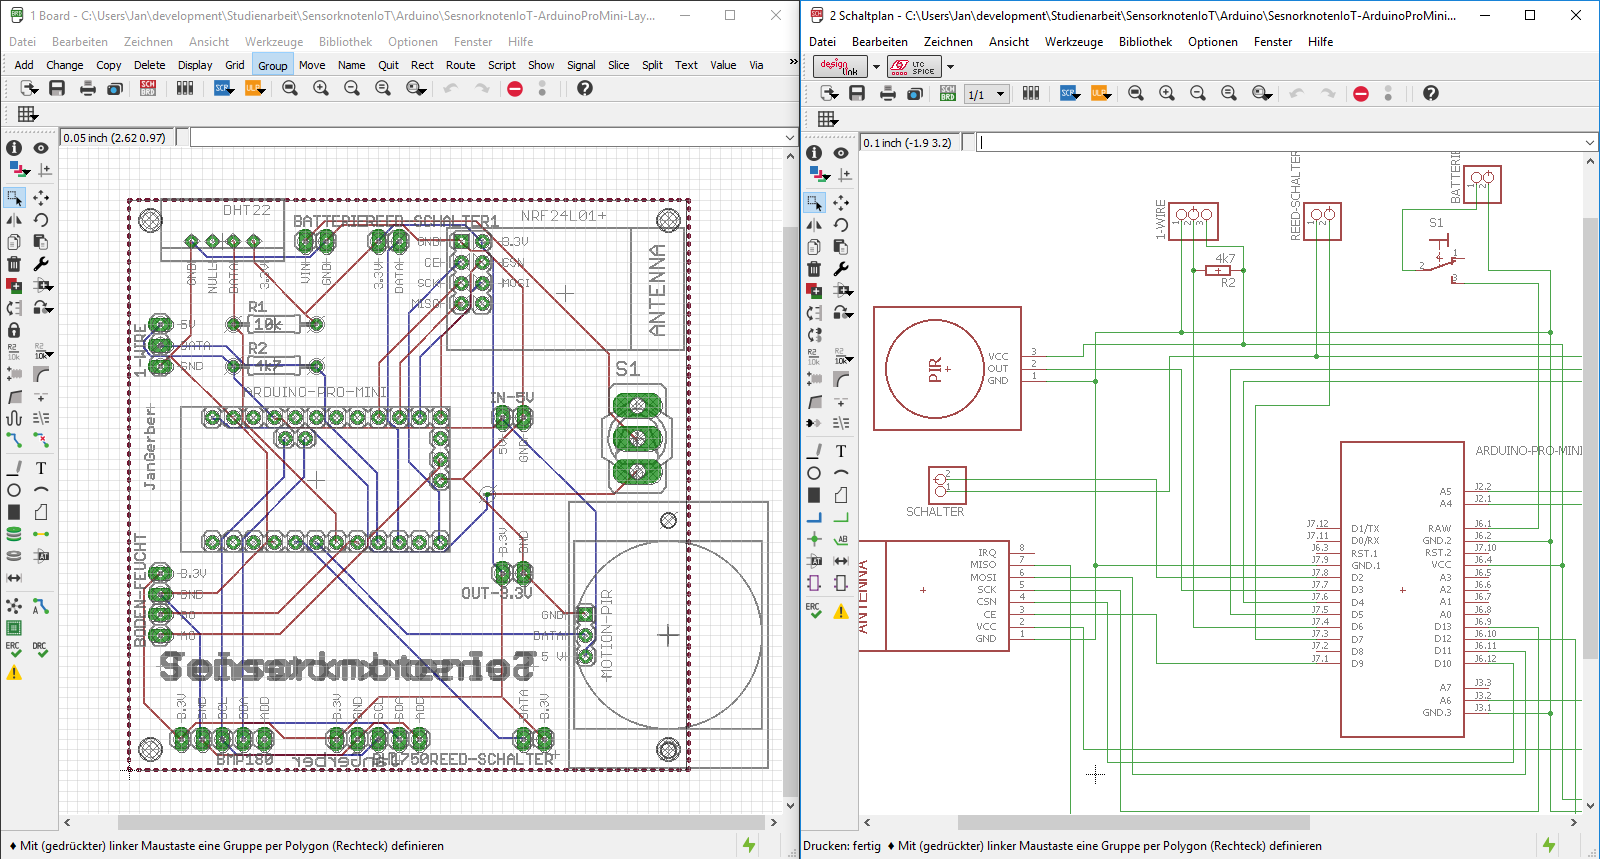
\includegraphics[width=1\textwidth]{bilder/Eagle}
	\caption[Eagle Autodesk – Layout Editor und Schaltplan Editor]{Eagle Autodesk – Layout Editor (linke Bildhälfte) und Schaltplan Editor (rechte Bildhälfte)}
	\label{img:EagleAutodesk}
\end{figure}
